\chapter{Wstęp}
\label{chapter:intro}

W~ramach pracy rozpatrywany jest problem weryfikacji postępów prac studentów dla projektu informatycznego, gdzie mamy zdefiniowane kilka grup projektowych.
Każdy z~zespołów, podczas trwania semestru, wykonuje taki sam rodzaj projektu.
Studenci przybliżają się do jego ukończenia poprzez zaliczanie kolejnych etapów.
Przykładem takiego projektu jest między innymi zadanie wykonywane w~ramach przedmiotu ”Podstawy Programowania” prowadzonego na wydziale Elektroniki i~Technik Informacyjnych w~realizacji zima 2018.

W pierwszym podrozdziale omówiono potrzebę oraz korzyści płynące z~przeprowadzania projektów grupowych w~ramach programu studiów.
Przedstawiony również został kierunek, w~jakim będą zmierzać przedmioty projektowe w~myśl reformy edukacji z~roku 2018.

Kolejny podrozdział opisuje problemy, na jakie mogą napotkać prowadzący oraz studenci podczas uczestnictwa w~projekcie grupowym.

Podrozdział \ref{tools} zawiera przegląd dostępnych, istniejących narzędzi wspomagających weryfikację umiejętności programistycznych użytkowników oraz ich zastosowanie w~branży informatycznej.

W sekcji \ref{programs-testing} omówiono sposoby oceny prawidłowości działania aplikacji.
Opisano tam również potrzebę nauki umiejętności testowania aplikacji przez studentów studiów informatycznych.

W ostatniej sekcji zostało zamieszczone podsumowanie oraz wnioski.


\section{Projekty grupowe}

Prowadzenie projektów grupowych niesie ze sobą wiele korzyści.
Na podstawie obserwacji obecnego rynku IT (ang. Information Technology) można stwierdzić, że większość komercyjnych projektów to projekty zespołowe.
Uczestnicząc w~projekcie grupowym w~ramach zajęć, student przystosowuje się do warunków, z~jakimi zetknie się w~swojej pierwszej pracy.

Projekt zespołowy pozwala na naukę pracy w~grupie.
Wymusza na studentach komunikację zarówno z~członkami zespołu, jak i~z prowadzącym.
Kształtuje umiejętność analizy, właściwego podziału zadań oraz estymacji czasu ich wykonania.
Studenci uczą się również odpowiedzialności nie tylko za swoją pracę, ale również za efekty całego zespołu.
Niejednokrotnie biorą też udział w~rozwiązywaniu konfliktów w~grupie.
Wszystkie powyżej wymienione kompetencje są istotne podczas pracy zawodowej.


Umiejętność pracy w~grupie jest bardzo pożądana przez pracodawców.
W ramach pracy \cite{soft-skills} zgrupowano i~poddano ocenie miękkie umiejętności, jakimi powinni posługiwać się pracownicy branży IT.
Badania zostały przeprowadzone na podstawie analizy wymagań zawartych w~650 ofertach pracy z~uwzględnieniem różnych lokalizacji.
Wyróżniono cztery kategorie stanowisk: analityk systemowy, projektant oprogramowania, programista oraz tester.
Dla każdego ze stanowisk najczęściej wymaganą cechą jest komunikatywność.
Praca w~grupie jest kolejną wskazywaną miękką umiejętnością.
Jest ona ceniona wyżej niż samodzielność w~wykonywaniu zadań.
Zestawienie pożądanych umiejętności miękkich, jakimi powinni posługiwać się programiści, uzyskanych w~ramach pracy F.~Ahmed zostało przedstawione na rysunku \ref{fig:soft-skills}.

\begin{figure}[h]
    \centering
    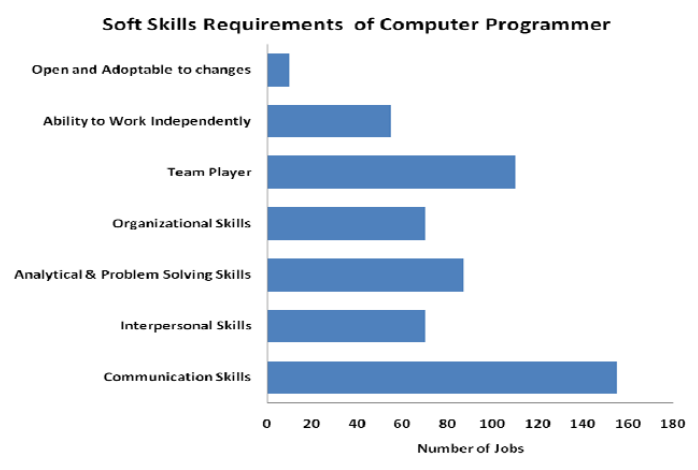
\includegraphics[width = 13cm]{chapter02/soft-skills.png}
    \caption{Pożądane umiejętności miękkie, jakimi powinni posługiwać się programiści (źródło \cite{soft-skills}).}
    \label{fig:soft-skills}
\end{figure}

Również wśród czterech wartości będących filarami metodyki Agile, zawartymi w~manifeście \cite{agile-manifesto} będącym publiczną deklaracją wrażającą koncepcję zwinnego podejścia do wytwarzania oprogramowania, połowa z~nich odnosi się bezpośrednio do komunikacji.
W~myśl tych dwóch założeń podejście Agile przedkłada ludzi i~interakcje ponad narzędzia i~procesy oraz współpracę z~klientem ponad negocjacje umów.
Umiejętność komunikacji można szlifować zarówno przez wspólną pracę w~ramach zespołu, jak i~dialog z~prowadzącym.

Korzyści z~projektów grupowych nie odnoszą się tylko do polepszenia umiejętności miękkich uczestników projektu.
Z założenia grupę projektową tworzą różne osoby, z~których każda ma inne, własne zaplecze wiedzy technicznej.
Poprzez pracę w~grupie studenci mają możliwość wymienienia się swoimi doświadczeniami i~wiedzą.
Co więcej, mogą spojrzeć na ten sam, zadany problem z~różnych perspektyw i~dojść do odrębnych wniosków.
Może to znacznie skrócić czas wykonania zadania i~wyeliminować błędy na wczesnym etapie. 
Wymiana doświadczeń i~dyskusje na temat różnych podejść do zadanego problemu mogą również rzutować na lepsze podejście do rozwiązywania zadań w~przyszłości.

W myśl ustawy ”Prawo o~szkolnictwie wyższym i~nauce” z~dnia 20 lipca 2018 \cite{higher-education-law}, od semestru zima 2019, w~ramach programu studiów będzie kładziony nacisk na prowadzenie projektów grupowych.
Jest to podyktowane dążeniem do zapewnienia wysokiej jakości kształcenia oraz właściwego przygotowania do wykonywania zawodu.

Wspieranie i~rekomendowanie prowadzenia projektów grupowych nie jest promowane jedynie w~Polsce.
Jest to aktualnie dominująca koncepcja kształcenia dla wiodących uczelni technicznych na świecie.
Jako przykład można podać Amerykańską Uczelnię MIT (ang. Massachusetts Institute of Technology), na której stronie internetowej można znaleźć następujący komunikat kierowany do kandydata:

\textit{”The core of the MIT spirit is collaboration and cooperation; you can see it all over the Institute.
Many of the problem sets (our affectionate term for homework) at MIT are designed to be worked on in groups, and cross-department labs are very common.
MIT is known for its interdisciplinary research.
If you enjoy working alone all the time, that’s completely valid, but you might not be particularly happy at MIT.”} \cite{mit-groups}.

W myśl tego komunikatu student wydziału powinien być otwarty na współpracę i~realizowanie projektów grupowych.

Opieranie nauki na prowadzeniu projektów zespołowych jest zatem pożądanym trendem przystosowującym studentów do przyszłej pracy zawodowej.
Jednak wykonywanie grupowych zadań niesie ze sobą wiele problemów.
Możemy wśród nich wyróżnić między innymi kłopoty z~prawidłową oceną zespołu i~poszczególnych członków wchodzących w~jego skład  oraz trudności związane z~podtrzymywaniem motywacji.
Obecny proces weryfikacji pracy studentów oraz napotykane problemy zostaną szerzej omówione w~kolejnym podrozdziale.

\section{Problemy związane z~weryfikacją pracy studentów}

Jak zostało wspomniane w~poprzednim podrozdziale, opieranie nauki na prowadzeniu projektów zespołowych jest bardzo pożądanym podejściem.
Praca grupowa ma jednak swoje wymagania.
Należą do nich między innymi: odpowiednia komunikacja, wypracowanie metod współpracy, właściwe ocenianie rezultatów oraz wkładu poszczególnych członków zespołu.
Dotychczasowy model edukacji promował indywidualizację.
W celu właściwego przeprowadzenia projektu zespołowego należy zmienić pewne nawyki i~wypracować nowe podejście zadowalające zarówno studentów, jak i~prowadzących.

Obecnie proces weryfikacji pracy studentów nad projektem zespołowym podczas semestru jest czasochłonny.
Każdy z~prowadzących ma pod swoją opieką kilka grup projektowych.
W skład każdego z~zespołów wchodzi kilku studentów.
Projekt jest podzielony na etapy, czasem wymaga wzajemnej integracji modułów napisanych przez różnych członków zespołu.
Te powyższe czynniki sprawiają, że praca w~ramach grupowego projektu, zarówno od strony prowadzącego, jak i~studentów, jest dość rozciągnięta w~czasie i~wymaga realizacji wielu podzadań.

Pomimo powtarzalności problemów, jakie mają do wykonania poszczególne zespoły i~definicji wymagań przez prowadzących, przekazywanych razem z~opisem projektu, rozwiązania tworzone przez studentów są zupełnie różne.
Zespoły często też błędnie interpretują i~implementują założenia.
Przy ocenie postępów prowadzący bazuje na prezentacji programu wykonanej przez studentów lub na własnych doświadczeniach z~interakcji z~programem.
W wyniku tego poszczególne zadania wykonywane przez studentów muszą być oceniane indywidualnie.
Sprawia to, że proces weryfikacji wydłuża się.

Przedstawienie prowadzącemu wyników cząstkowych oraz końcowych przez studentów może okazać się kłopotliwe.
Manualne uruchamianie programów na prywatnych maszynach studentów jest czasochłonne.
Dodatkowo podczas przedstawiania wyników, mogą zaistnieć komplikacje związane między innymi z~niepoprawną konfiguracją środowiska uruchomieniowego lub niewłaściwym doborem przypadków testowych.
W sytuacji, gdy zadaniem studentów jest zaprezentowanie interakcji pomiędzy stworzonymi przez nich modułami programów, prawdopodobieństwo wystąpienia powyższych błędów wzrasta.
Prowadzący, decydując się na samodzielne uruchomienie programów studentów, w~celu ich oceny, jest również narażony na powyższe sytuacje.
W przypadku niedokładnej dokumentacji dotyczącej pracy studentów, jego zadanie może zostać znacznie utrudnione.
Taka sytuacja może doprowadzić do uzyskania niskiego wyniku przez studentów mimo niewielkich błędów w~implementacji lub błędnie zrozumianych założeń.
Podejście prowadzącego do każdego z~zespołów i~etapów jest indywidualne.

Studenci otrzymują informację dotyczącą oceny danego etapu po jego zakończeniu.
W trakcie zadania oczywiście mogą doprecyzować szczegóły z~prowadzącym.
Zdarza się jednak, że pomimo dodatkowego uszczegółowienia, niektóre założenia są przez studentów zrozumiane w~inny sposób niż oczekiwałby tego prowadzący.
W takim przypadku studenci podczas trwania etapu mogą napisać program zgodny z~błędnie rozumianymi założeniami i~dopiero po złożeniu kompletnego sprawozdania z~etapu dowiedzieć się o~niepoprawnej interpretacji zadania.
Zatem kolejnym napotykanym problemem może być uzyskanie miarodajnej informacji zwrotnej w~odpowiednio krótkim czasie.

Podczas prowadzenia projektu prowadzący napotykają również na problem braku systematycznej pracy studentów podczas semestru.
Może on być częściowo rozwiązany poprzez dostęp do wiedzy o~aktualnych postępach innych grup, na co wskazują coraz liczniej formułowane postulaty gamifikacji procesu nauczania \cite{gamification}.
Podgląd statusu prac pozostałych zespołów mógłby być dodatkową motywacją dla studentów do podjęcia działań i~wykonania danego etapu.

Proces prowadzenia projektów grupowych jest aktualnie modernizowany.
Dla przedmiotu ”Podstawy Programowania” wśród wprowadzanych usprawnień można wyróżnić między innymi zobligowanie studentów do zamieszczania kodu swoich aplikacji w~systemie kontroli wersji GitLab.
Jest to istotna modernizacja pozwalająca na lepsze zarządzanie kodem programów i~jego archiwizację.
Jednak studenci (zwłaszcza pierwszych lat studiów) nie potrafią w~pełni wykorzystać zalet tego narzędzia i~poprawnie z~niego korzystać.
Często nie zamieszczają kodu w~postaci małych czytelnych tzw. ”commit'ów”.
Zamiast tego zamieszczają całe archiwa z~nowymi wersjami oprogramowania.
Dokumentacja programów również nie jest zawsze pełna.
Usprawnienie w~postaci systemu kontroli wersji ułatwia dostęp do kodu programów studentów i~pozwala przeglądać go na przystosowanym do tego interfejsie.
Nie eliminuje to jednak czasochłonnego, indywidualnego podejścia do oceny każdej z~grup i~etapu.

Dzięki wprowadzeniu systemu kontroli wersji można uzyskać szereg statystyk dotyczących pracy studentów.
Nie są to jednak pełne informacje, które mogłyby interesować prowadzącego.
Sam kod zamieszczany w~systemie, nie jest wystarczający do oceny etapu.
Co więcej, jego samodzielna analiza nie poprawiłaby, a być może nawet pogorszyła, czasochłonność weryfikacji wyników cząstkowych.
Ważnym elementem oceny poszczególnych etapów jest ocena poprawności działania uruchomionych programów dla zadanych danych wejściowych.

Obecnie dostępne jest wiele narzędzi wspomagających proces nauki programowania oraz ocenę umiejętności programistycznych.
Ich koncepcje oraz ograniczenia co do wykorzystania w~ramach wieloetapowego zespołowego projektu informatycznego zostaną omówione w~kolejnym podrozdziale.


\section{Narzędzia wspomagające ocenę umiejętności programistycznych}
\label{tools}

Obecnie istnieje wiele narzędzi wspomagających ocenę umiejętności programistycznych użytkowników.
Są to najczęściej ogólnodostępne platformy z~interfejsem webowych.
Główna zasada działania tych narzędzi sprowadza się do napisania przez użytkownika prostego, odseparowanego programu z~zadaną wejściową sygnaturą.
Następnie kod jest kompilowany, budowany i~przepuszczany przez szereg testów akceptacyjnych.
Wynik testów jest przedstawiany użytkownikowi w~postaci prostej wizualizacji.

Wśród narzędzi można wyróżnić strony umożliwiające testowanie umiejętności algorytmicznych użytkowników.
Pozwalają one zarówno na sprawdzenie poprawności wykonania implementowanych algorytmów, jak i~ocenę ich złożoności.
Umożliwiają one także przeprowadzanie zawodów w~szybkim tworzeniu poprawnych i~efektywnych algorytmów.
Do takich rozwiązań należą między innymi: Codility \cite{codility} i~HackerRank \cite{hacker-rank}.
Słuszność takich platform można potwierdzić między innymi na podstawie tego, że duże międzynarodowe korporacje takie jak Google zachęcają do przygotowywania się do procesów rekrutacyjnych z~użyciem stron tego rodzaju.
Niektóre mniejsze firmy prowadzą początkowe etapy rekrutacji z~wykorzystaniem tych platform.

Kolejnym rodzajem narzędzi są strony umożliwiające naukę programowania lub naukę programowania we wskazanym języku.
Mogą być to proste symulatory środowisk, gdzie wraz z~kolejnym etapem kursu użytkownik ma za zadanie napisać niewielki program lub jego część.
Czasem jednak narzędzia są bardziej rozbudowane i~pozwalają na wizualizację działania programów w~formie gry np. CodinGame \cite{game-coder}.
Podejście z~tworzeniem gier jest wykorzystywane w~celu zachęcenia i~zainteresowania użytkowników oraz lepszego zobrazowania wyniku działania ich kodu.
Wśród narzędzi mających na celu lepsze zrozumienie wykonania kodu przez wizualizację można wyróżnić platformę do nauki programowania równoległego opisaną w~artykule \cite{pharaller-platform}.

Wprowadzenie takich narzędzi do pomocy w~procesie nauki programowania dla zespołowego projektu informatycznego w~ramach przedmiotu uczelnianego jest jednak utrudnione.
Wspomniane platformy służą do oceny poprawności pojedynczych, niewielkich fragmentów kodu i~nie da się użyć ich do weryfikacji pełnego projektu informatycznego.
Ze względu na powyższe cechy użycie ich w~ramach wieloetapowego, długoterminowego i~grupowego projektu nie pomoże znacząco usprawnić procesu weryfikacji pracy studentów.
Dodatkowo z~założenia użytkownikiem powyższych platform jest pojedyncza osoba.
Nie są one przystosowane do zarządzania wspólnym zasobem (projektem) przez grupę.
Innym z~problemów jest między innymi to, że bardzo często firmy zarabiają na udostępnianiu licencji do korzystania z~tych rozwiązań.
Stąd wprowadzenie tych narzędzi na dużą skalę generowałoby dodatkowy koszt.

Tworzenie platform pozwalających studentom na poszerzanie umiejętności programistycznych jest rozwijanym i~szeroko stosowanym trendem.
W ramach pracy doktorskiej \cite{teach-testing-thesis} opisano narzędzie pozwalające na naukę pisania testów jednostkowych.
Bazując na danych historycznych, zaproponowano platformę pozwalającą na ocenę jakości testów pisanych przez użytkowników.
Jest to bardzo ciekawe i~godne uwagi podejście do oceny umiejętności testowania programów przez studentów.

Narzędzia wspomagające ocenę umiejętności programistycznych są powszechne i~mają różne zastosowania.
Wspólnymi cechami rozwiązań są między innymi: ogólnodostępność, posiadanie interfejsu webowego, zorientowanie na pojedynczego użytkownika.
Sposób sprawdzania poprawności działania kodu napisanego w~ramach zadań na platformach jest również podobny.
Polega on na przeprowadzeniu szeregu zdefiniowanych wcześniej dla problemu automatycznych testów akceptacyjnych.

Na podstawie analizy rozwiązań można wywnioskować, że dzisiejsi użytkownicy (w~tym studenci) chętnie pracują w~chmurze, są zorientowani wizualnie oraz liczą na wsparcie w~pracy od strony technologicznej i~możliwość szybkiego wprowadzania zmian.
Wszystko to wynika z~dzisiejszej rzeczywistości biznesowej, ciągle się zmienia i~oferuje nowe ciekawe rozwiązania technologiczne.

W kolejnym podrozdziale omówiono sposób weryfikacji prawidłowości zachowania aplikacji przy użyciu testów manualnych oraz automatycznych.
Rozpatrzono również aktualne trendy co do potrzeby posiadania umiejętność testowania kodu przez programistów.


\section{Testy jako sposób oceny działania aplikacji}
\label{programs-testing}

W ramach podrozdziału \ref{test_practices} omówiono dobrą praktykę wykorzystywaną w~procesie wytwarzania oprogramowania, jaką jest automatyczne testowanie kodu.
Sekcja \ref{test_studies} opisuje potrzebę wprowadzenia nauki testowania aplikacji w~ramach programu studiów i~związane z~tym trudności.
W ostatnim podrozdziale omówiono również aktualnie badane podejścia służące do weryfikacji poprawności programów studentów poprzez wykonanie testów automatycznych.

\subsection{Testy jako element procesu wytwarzania oprogramowania}
\label{test_practices}

Ważnym elementem procesu wytwarzania oprogramowania jest zweryfikowanie poprawności jego działania.
Ocenę prawidłowość działania aplikacji można przeprowadzić manualnie, jednak zazwyczaj jest to bardzo czasochłonny proces.
Dodatkowo rezultat ręcznej weryfikacji jest obarczony dużym błędem wynikającym z~czynnika ludzkiego związanego z~niewłaściwym działaniem człowieka, które skutkuje przekłamaniem wyników.
Przykładem takiego błędu może być przykładowo omyłkowe użycie niepoprawnego pliku wejściowego.

Na rysunku \ref{fig:tests-levels} zostały przedstawione poziomy testów.
Ze względu na czasochłonność dla procesu wytwarzania oprogramowania wskazane jest, aby testy manualne stanowiły niewielki procent wszystkich testów aplikacji.
Zatem nacisk powinno się kłaść na automatyczne przeprowadzanie weryfikacji programów.

\begin{figure}[h]
    \centering
    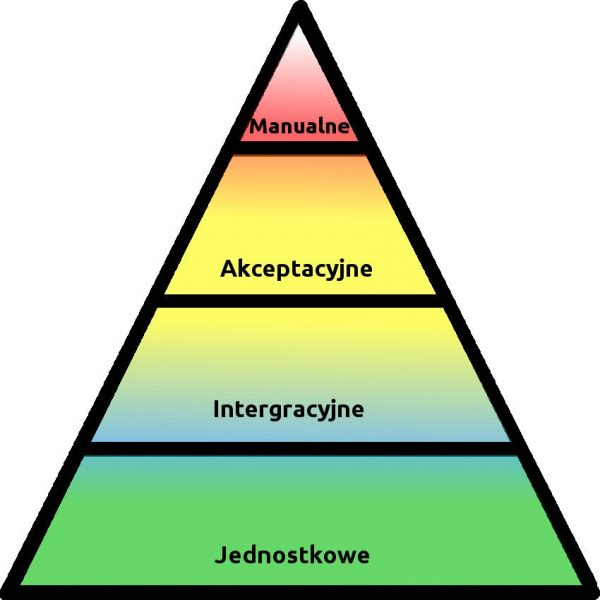
\includegraphics[width = 5cm]{chapter02/tests_levels.jpg}
    \caption{Poziomy testów (źródło: \cite{tests-levels}).}
    \label{fig:tests-levels}
\end{figure}

Na podstawie wyników ankiety portalu Stack Overflow z~roku 2019 widać, że umiejętność testowania kodu jest bardzo istotna w~przyszłej pracy \cite{stack-overflow-survey}.
W ramach badania zapytano ankietowanych, czy w~ich miejscach pracy używa się testów jednostkowych podczas wytwarzania oprogramowania.
Na rysunku \ref{fig:unit-tests-use} przedstawiono wyniki ankiety.
W~przybliżeniu jeden na trzech ankietowanych nie używa testów najniższego poziomu w~swoim procesie, ale zaledwie 4.4\% jest zadowolona z~takiego podejścia.
95.6\% osób testuje jednostkowo swoje aplikacje lub uważa, że ten rodzaj testów byłby przydatny w~procesie wytwarzania oprogramowania.
Warty uwagi jest również rezultat otrzymany w~powiązaniu używania testów jednostkowych z~poziomem satysfakcji z~pracy ankietowanych, który został przedstawiony na rysunku \ref{fig:unit-tests-satisfaction}.
Osoby używające tego rodzaju testów są bardziej zadowolone ze swojej pracy.

\begin{figure}[h]
    \centering
    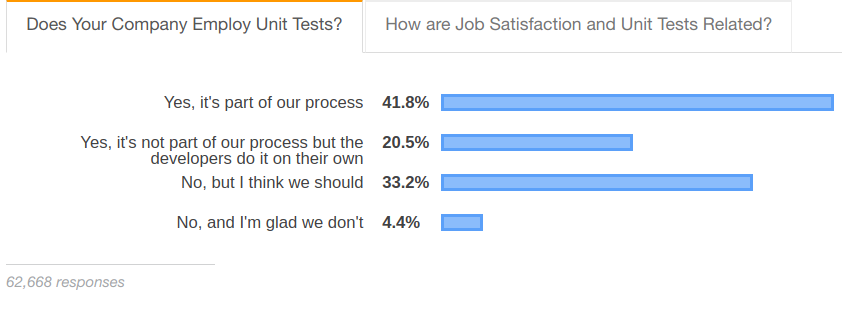
\includegraphics[width = 13cm]{chapter02/unit-tests-use.png}
    \caption{Używanie testów jednostkowych w~procesie wytwarzania oprogramowania (źródło: \cite{stack-overflow-survey}).}
    \label{fig:unit-tests-use}
\end{figure}

\begin{figure}[h]
    \centering
    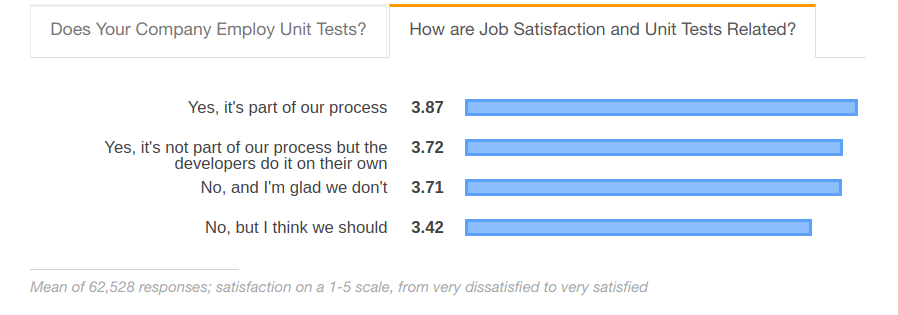
\includegraphics[width = 13cm]{chapter02/unit-tests-satisfaction.png}
    \caption{Powiązanie używania testów jednostkowych i~zadowolenia z~pracy (źródło: \cite{stack-overflow-survey}).}
    \label{fig:unit-tests-satisfaction}
\end{figure}

Umiejętność testowania kodu jest często sprawdzana podczas procesu rekrutacyjnego.
Zarówno w~przypadku, gdy kandydat ma za zadanie zaimplementować małe zdanie algorytmiczne, jak i~napisać działającą aplikację.
W obu przypadkach musi on udowodnić poprawność swojego rozwiązania poprzez testy.
Niezależnie czy poprzez analizę słowną przebiegu działania programu, czy przez zaimplementowane testy wewnątrz aplikacji.
W~pozycji pomagającej przygotować się do procesu rekrutacji ”Cracking the coding interview” \cite{cracking-the-coding-interview} testowaniu został poświęcony odrębny rozdział.

Programiści ćwiczący umiejętność testowania aplikacji potrafią lepiej wychwytywać potencjalne błędy na wczesnym etapie tworzenia oprogramowania.
W przypadku małych i~średnich firm wytwarzających oprogramowanie z~wykorzystaniem podejścia Agile, często nie ma oddzielnych zespołów testerów.
W takich software house'ach zadaniem inżyniera oprogramowanie jest nie tylko napisanie działającej funkcjonalność, ale również samodzielne przetestowanie jej poprzez testy jednostkowe i~integracyjne.
W dużych korporacjach wykorzystujących metodyki Agile umiejętność testowania jest również istotna ze względu na ścisłą współpracę między interdyscyplinarnymi członkami zespołu.

Wśród wartości fundamentalnych dla podejścia XP (ang. Extreme Programming) do wytwarzania oprogramowania jest wymieniona informacja zwrotna (ang. feedback) \cite{extreem-programming}.
Opisywana jest ona jako szybkość oceny poprawności dodawanego kodu i~jego interakcji z~innymi częściami systemu oraz oszacowania regresji.
Szybką informację zwrotną dotyczącą dodawanej funkcjonalności można osiągnąć między innymi przez utrzymywanie poprawnych przypadków testowych.

\subsection{Wprowadzanie nauki umiejętności testowania aplikacji do programu studiów}
\label{test_studies}

W literaturze można znaleźć wiele prac poświęconych testowaniu programów i~wprowadzaniu nauki umiejętności testowania w~ramach programu studiów.
Kładziony jest coraz większy nacisk na tę umiejętność \cite{tests-important}.
Wśród zamieszczonych opinii powszechną jest, że testowanie aplikacji jest ważne i~potrzebne od samego początku studiów \cite{test-from-scratch}.
Pośród propozycji można znaleźć pomysł nauki pisania programów w~metodyce TDD (ang. Test Driven Development) \cite{tdd-on-start}.
Wymagałoby to jednak wysokich kwalifikacji prowadzących co do znajomości metodyki i~jej praktyki.
Warto zaznaczyć, że TDD opiera się na pisaniu testów jednostkowych, co wymaga wiedzy na temat programowania.

Zatem w~ramach weryfikacji programów studentów można byłoby oczekiwać, że studenci sami tworzyliby testy automatyczne dla swoich aplikacji.
Podczas prezentacji programów prowadzącemu do ich zadania należałoby udowodnić, że kończą się one pozytywnym wynikiem.
Niestety ciężko ocenić trafność napisanych przez studentów przypadków testowych.
Podjęcie się takiego zadania przez prowadzącego wymagałoby od niego jeszcze bardziej indywidualnego podejścia do weryfikacji pracy grupy niż obecnie, w~przypadku sprawdzenia wyniku działania samego programu.
Jest to związane między innymi z~tym, że część napisanych przez studentów testów mogłaby się powtarzać lub być nieprawidłowa.
Aby poprawnie ocenić jakość przypadków testowych należałoby rozważyć  między innymi priorytetyzajcę testowanych funkcjonalności, użyte narzędzia i~poprawność asercji.
Samo zadanie napisania testów dla tworzonego programu mogłoby się okazać wyjątkowo ciężkie do zrealizowania w~przypadku studentów, którzy są dopiero na początku swojej kariery programistycznej.
Takie osoby dopiero uczą się struktur języka i~bardzo często nie mają wystarczająco dużo wiedzy, aby napisać poprawnie testy~\cite{tests-and-begginers}.

Zatem studentom rozpoczynającym naukę programowania bardzo ciężko byłoby napisać odpowiednie testy do swoich programów.
Praktycznie niemożliwe jest też wprowadzenie na początku studiów całego przedmiotu poświęconego nauce pisania testów, ze względu na przepełniony obecnie program studiów \cite{overflow-studies-program}.
Warto jednak pokazywać studentom zalety testowania aplikacji.
Można to osiągnąć między innymi przez dostarczanie studentom zdefiniowanych przez prowadzących poprawnych przypadków testowych dla ich programów.

W zależności od poziomu złożoności aplikacji wysokie pokrycie testowe mogłoby być jednak trudne do utrzymania.
Wraz ze wzrostem skomplikowania programów tworzenie przypadków testowych przez prowadzących stawałoby się coraz bardziej czasochłonne.

Ciekawym pomysłem zmniejszenia czasu potrzebnego na dodawanie testów jest zobligowanie studentów do samodzielnego pisania przypadków testowych, zebranie wszystkich testów i~uruchomienie programu każdej grupy dla wszystkich zebranych przypadków.
Słuszność takiego podejścia została opisana w~artykule \cite{write-tests-by-students}.
Warto jednak zaznaczyć, że zadaniem prowadzącego w~tym przypadku byłaby ocena jakości przypadków testowych.
Dodatkowo mogłoby się okazać, że zbiór testów ma stosunkowo niskie pokrycie, co jest wysoce prawdopodobne w~przypadku studentów rozpoczynających naukę programowania.
Można jednak oczekiwać, że im większe doświadczenie studentów, tym lepsze pokrycie testami aplikacji osiągniemy.

Innym pomysłem na zmniejszenie czasochłonności tworzenia testów automatycznych jest porównywanie wyników programów studentów ze wzorcowym programem prowadzącego uruchomionym dla tych samych danych wejściowych.
W tym przypadku dane wejściowe mogłyby być generowane losowo.
Ten sposób chroniłby przed próbą sztywnej implementacji programu, która generowałaby właściwy wynik tylko dla znanych wcześniej przypadków testowych.
To podejście ma też swoje wady, ponieważ używając zwykłego generatora losowego można uzyskać bardzo niskie pokrycie i~nie przetestować poprawnie przypadków brzegowych.

Kolejnym innowacyjnym podejściem jest wykorzystanie metod ML (ang. Machine Learning) do generowania przypadków testowych.
Ta metoda została opisana we wspomnianej wcześniej pracy doktorskiej~\cite{teach-testing-thesis}.
Dzięki uczeniu maszynowemu z~wykorzystaniem prac studentów z~poprzednich lat uzyskano narzędzie pozwalające generować przypadki testowe z~bardzo wysokim pokryciem.



\section{Podsumowanie}

Prowadzenie informatycznych projektów zespołowych w~celu nauki programowania niesie ze sobą wiele korzyści.
Studenci biorąc udział w~takich zajęciach są przystosowani lepiej do warunków, które spotkają w~przyszłej pracy.
Prowadzenie projektów grupowych jest aktualnym trendem zarówno w~Polsce, jak i~na świecie.

Jednak dotychczasowy model edukacji promował indywidualizację.
Aby uzyskać w~pełni korzyści płynące z~prowadzenia grupowego projektu wymagane jest wpracowanie nowych metod współpracy pomiędzy prowadzącym a studentami.
Obecny proces weryfikacji pracy studentów w~ramach zadania zespołowego jest czasochłonny ze względu na indywidualne podejście do każdej z~grup i~podzadań.

Obecnie istnieje wiele narzędzi wspomagających naukę programowania.
Te narzędzia przystosowane są jednak do indywidualnej pracy dla niewielkich i~pojedynczych zadań, przez to trudno wykorzystać je do usprawnienia weryfikacji pracy grupowej.

Wspomniane narzędzia wykorzystują testy w~celu oceny poprawności działania programów.
Automatyczna weryfikacja kodu jest dobrą praktyką dla procesu wytwarzania oprogramowania i~w ramach studiów informatycznych kładziony jest coraz większy nacisk na naukę umiejętności testowania aplikacji.

Jednak wymaganie od studentów, zwłaszcza na początkowym etapie studiów, samodzielnego pisania testów automatycznych jest trudne do zrealizowania, ponieważ nie znają oni dobrze struktur języków programowania.
Napisane przez nich przypadki testowe uzyskałyby bardzo niskie pokrycie.
Warto jednak uświadamiać studentom zalety testowania aplikacji i~pokazać dobre praktyki w~pisaniu testów i~sprawdzaniu warunków brzegowych.

Na podstawie analizy zagadnienia w~ramach pracy zaprojektowano i~zbadano platformę usprawniającą proces weryfikacji zespołowego projektu informatycznego.
Kluczowa koncepcja platformy opiera się na wykorzystaniu zestawu testów akceptacyjnych do weryfikacji pracy studentów.
Dzięki takiemu podejściu możliwe jest osiągnięcie wielu korzyści takich jak ograniczenie indywidualnego podejścia do grup, zmniejszenie czasochłonności procesu weryfikacji, uzyskanie dostępu do bieżącej informacji zwrotnej z~rezultatem uruchomienia programów.

Platforma proponowana w ramach pracy jest dostosowana do wymagań pracy zespołowej między innymi przez udostępnienie studentom wchodzącym w~skład grupy zarządzania zasobami całego zespołu.
Narzędzie może być również użyte w~przypadku projektu indywidualnego.

Rozwiązanie wychodzi naprzeciw oczekiwaniom studentów, udostępniając webowy interfejs i~wspierając proces ich pracy od strony technologicznej.
Proponowane rozwiązanie jest generyczne i~poprzez odpowiednie zdefiniowanie środowiska uruchomieniowego może zostać użyte dla dowolnego języka programowania na każdym etapie studiów.


Pełna koncepcja platformy została opisana w~kolejnym rozdziale.




